\chapter{Estudo Piloto} \label{capitulo:estudo-piloto}

O objetivo do estudo piloto conduzido, foi avaliar se uma rede neural convolucional treinada em dados sintéticos gerados por um modelo de difusão, teria desempenho similar a uma rede treinada em dados reais nas medidas de acurácia, sensibilidade, precisão e F1. As próximas seções trarão ao leitor detalhes sobre o conjunto de dados utilizado, a metodologia empregada, resultados parciais obtidos e as considerações sobre os resultados parciais.

\section{Conjunto de dados}

Para a realização do estudo piloto, foi utilizado o conjunto de dados \textit{Chest X-Ray Images (Pneumonia)}. Este conjunto possui um total de 5863 imagens de raio-x de tórax divididas previamente em conjuntos de treinamento, validação e teste.

O conjunto de treinamento possui 1341 imagens de pulmões saudáveis e 3875 imagens de pulmões com pneumonia. Já o conjunto de validação possui 8 imagens pertencentes a cada classe. Por sua vez, o conjunto de testes possui 624 imagens, sendo 234 de pulmões saudáveis e 390 de pulmões com pneumonia, a figura \ref{fig:xray-dataset-sample}.

\begin{figure}[htbp]
	\centering
	\caption[Exemplo de imagem do conjunto de dados \textit{Chest X-Ray Images}]{Exemplo de imagem do conjunto de dados \textit{Chest X-Ray Images}}
		\includegraphics[scale=.4]{imagens/xray-dataset-images.jpg}
	\label{fig:xray-dataset-sample}
  \source{\citeonline{xraychestdataset}}
\end{figure}

Para a execução dos experimentos deste estudo exploratório, as imagens foram redimensionadas para a resolução de 64x64 antes de serem utilizadas por um modelo gerador para a produção do conjunto de dados artificiais.

\section{Metodologia}

Para a execução dos experimentos, foi adotado o arcabouço comum de avaliação de modelos de classificação treinados em dados reais e dados sintéticos, já apresentado na figura \ref{fig:arcabouco-simples} do capítulo \ref{capitulo:introducao}. Três cenários de conjuntos de dados foram estabelecidos, sendo (a) conjunto de dados real, (b) conjunto de dados sintético com balanceamento igual ao real e (c) conjunto de dados sintético balanceado com sobre-amostragem da classe minoritária. Para a construção dos conjuntos de dados sintéticos, foi utilizado o modelo de difusão probabilístico proposto em \citeonline{ho_denoising_2020}. Para cada classe do conjunto de dados, um modelo gerador foi utilizado, de modo que somente os dados do conjunto de treinamento real fossem utilizados. A partir dos conjuntos sintéticos gerados, um conjunto de validação, de mesma proporção do conjunto real, foi extraído para posterior uso no modelo classificador. A figura \ref{fig:imagens-geradas} apresenta as amostras de imagens sintéticas geradas durante o treinamento dos modelos geradores.

\begin{figure}[htbp]
	\centering
	\caption[Exemplo do processo de aprendizado do modelo de difusão]{Exemplo do processo de aprendizado do modelo de difusão: A sequência das imagens mostra a evolução do aprendizado da remoção de ruído de uma imagem até que se pareçam com imagens do conjunto de dados de treinamento.}
		\includegraphics[scale=.25]{imagens/difussion-generated.jpg}
	\label{fig:imagens-geradas}
  \source{Alexandre Farias, 2024}
\end{figure}

O modelo classificador utilizado foi uma rede neural convolucional com três camadas de convolução utilizando a função de ativação ReLU, sendo que na primeira camada de convolução também foi adicionada uma camada de \textit{pooling} utilizando a média como função resumo. No bloco completamente conectado duas camadas ocultas foram utilizadas com 144 neurônios na primeira e 512 na segunda, sendo que na primeira camada oculta é aplicado um \textit{dropout} de 20\%. A saída da rede é composta por um único neurônio que utiliza a função sigmoide como função de ativação.

Para ajustar os pesos do modelo classificador, foi utilizado o método de gradiente descente estocástico, com taxa de aprendizado fixa igual a $10^{-3}$ com a função de perda de entropia cruzada binária. o número máximo de épocas definido para treinamento foi igual a 10 mil, com uma tolerância de 1200 épocas sem melhoria na medida F1 no conjunto de validação do respectivo cenário. Por fim, cada época consiste em ajustar o modelo com base em todo o conjunto de treinamento, mas submetido em lotes de 256 imagens por vez para a atualização dos pesos.

Por fim, para cada um dos cenários, 30 experimentos forma executados, totalizando o treinamento de 90 modelos de classificação, de cada experimento, as medidas de acurácia, sensibilidade, precisão e F1 foram armazenadas. Para o cálculo das métricas da matriz de confusão o limiar de classificação de 50\% foi adotado para todos os modelos. Em todos os três cenários, os modelos foram avaliados no conjunto de testes fornecido no conjunto de dados reais, nenhuma imagem sintética foi utilizada no conjunto de testes, para que o arcabouço contemple o cenário mais real possível de avaliação e evitar a superestimação da performance dos modelos.

Para validar a hipótese de que os modelos treinados em cada um dos cenários sintéticos possuem desempenhos similares ao modelos treinados no cenário real, o teste de \textit{Mann-Whitney} foi empregado para a comparação das medianas das distribuições, dado que a hipótese de normalidade foi rejeitada para todas as métricas em seus respectivos experimentos com $p < 0.05$.

Todo arcabouço foi implementado utilizando a linguagem de programação Python em conjunto de seu ecossistema de ferramentas estatísticas e para aprendizado de máquina.

\section{Resultados parciais}

Os resultados iniciais mostram que os modelos de classificação treinados nos dados sintéticos possuem desempenho similar e em alguns casos superior aos modelos treinados em dados reais, assim como observado na revisão bibliográfica. Em destaque, os modelos treinados em dados sintéticos balanceados foram melhores nas medidas de acurácia ($p < 0.01$), precisão ($p < 0.01$) e F1 ($p < 0.01$), quando comparados aos modelos reais.
Já os modelos treinados em dados sintéticos desbalanceados, tiveram desempenho médio inferior nas métricas de acurácia, precisão e F1, mas superior na métrica de sensibilidade, se comparados ao cenário de dados sintéticos balanceados, todavia, também apresentaram resultados satisfatórios quando comparados com modelos treinados no conjunto de dados real.
Por sua vez, os modelos treinados em dados reais apresentaram a melhor sensibilidade dentre todos os cenários de treinamento.
Os resultados dos experimentos podem ser conferidos em mais detalhes na tabela \ref{tab:estudo-piloto}

\begin{table}[htbp]
    \caption[Resultados dos experimentos realizados no estudo piloto]{Resultados dos experimentos realizados no estudo piloto: melhores resultados em cada métrica de avaliação destacados em negrito.}
    \resizebox{\textwidth}{!}{
        \begin{tabular}{@{}lllllllll@{}}
            \toprule
            &
            \multicolumn{2}{c}{\textbf{Acurácia}} &
            \multicolumn{2}{c}{\textbf{Precisão}} &
            \multicolumn{2}{c}{\textbf{Sensibilidade}} &
            \multicolumn{2}{c}{\textbf{F1}} \\ 
            \midrule
            Experimento &
            Média &
            Desvio Padrão &
            Média &
            Desvio Padrão &
            Média &
            Desvio Padrão &
            Média &
            Desvio Padrão
            \\
            XRAY-64x64-REAL &
            0.737 &
            0.055 &
            0.716 &
            0.046 &
            \textbf{0.970} &
            0.015 &
            0.716 &
            0.046
            \\
            XRAY-64x64-SYNTHETIC-UNBALANCED &
            0.764 &
            0.054 &
            0.762 &
            0.054 &
            0.920 &
            0.033 &
            0.762 &
            0.054
            \\
            XRAY-64x64-SYNTHETIC-BALANCED &
            \textbf{0.793} &
            0.015 &
            \textbf{0.823} &
            0.037 &
            0.857 &
            0.041 &
            \textbf{0.823} &
            0.037
            \\
            \bottomrule
        \end{tabular}
}
\label{tab:estudo-piloto}
\source{Alexandre Farias, 2024}
\end{table}

A figura \ref{fig:experimento-metricas} mostra a distribuição das métricas para os três cenários avaliados, em todas as métricas, algumas distribuições aparentam ser bimodais, este fenômeno é provavelmente explicado pela parada antecipada de modelos que levariam mais tempo para convergir para uma melhor solução.

\begin{figure}[htbp]
	\centering
	\caption[Distribuição das métricas da matriz de confusão no estudo piloto]{Distribuição das métricas da matriz de confusão no estudo piloto: enquanto o modelo treinado em dados reais possui a melhor sensibilidade, a utilização de um modelo treinado em um conjunto de dados de imagens sintéticas balanceado obteve melhores resultados nos outras métricas.}
		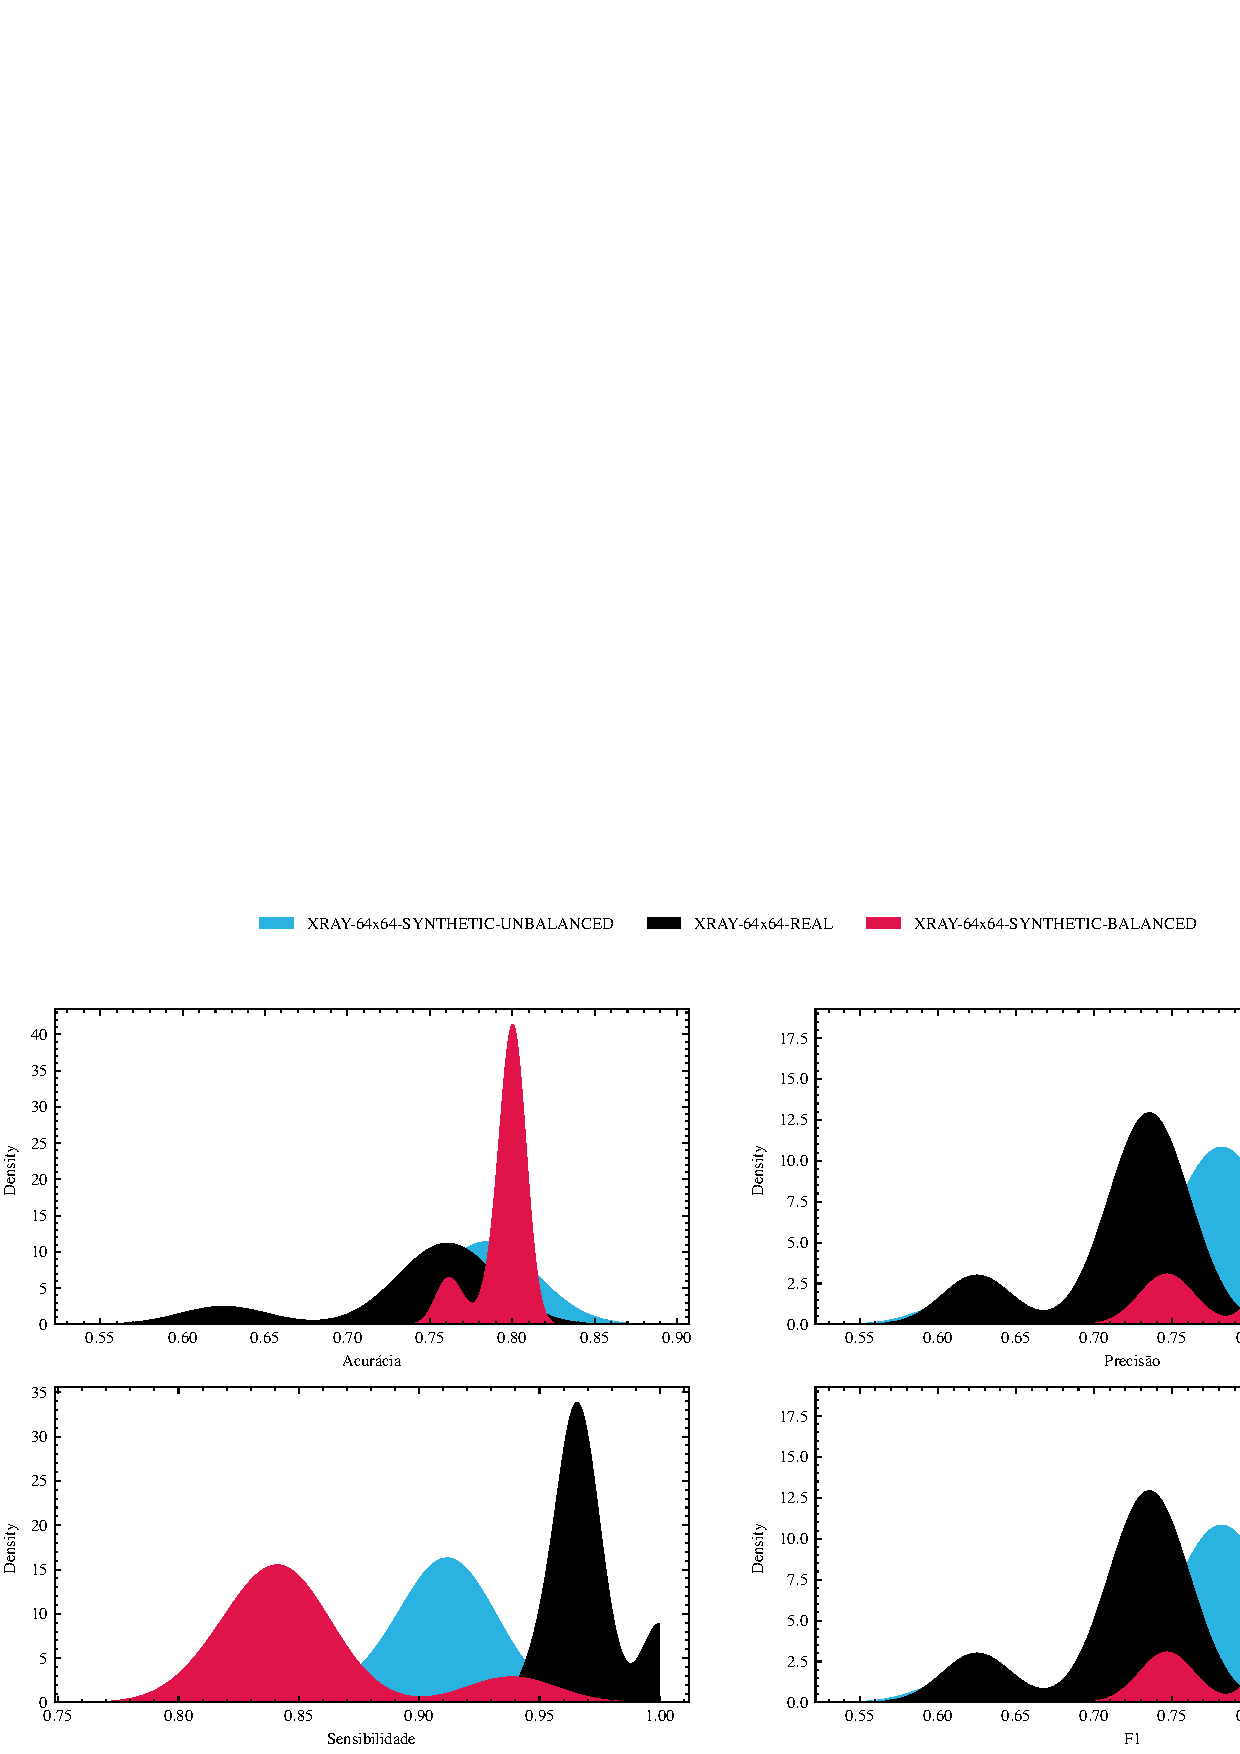
\includegraphics[scale=.9]{imagens/experimento-metricas-densidade.pdf}
	\label{fig:experimento-metricas}
  \source{Alexandre Farias, 2024}
\end{figure}

Dada a natureza desbalanceada do problema, a curva PR também foi avaliada para os modelos com maior medida F1 em cada cenário, a figura \ref{fig:experimento-pr} nos mostra os modelos treinados nos diferentes cenários possuem um desempenho similar, de modo que a variação do limiar de classificação permita a obtenção de classificadores treinados em dados sintéticos similares aos classificadores treinados em dados reais, como no caso dos modelos treinados em dados sintéticos desbalanceados. Por fim, a área sob a curva do modelo treinado em dados sintéticos balanceados se apresenta ligeiramente superior aos outros dois modelos, corroborando também com os resultados demonstrados previamente.

\begin{figure}[htbp]
	\centering
	\caption[Curva PR]{Curva PR: curvas apresentadas para os modelos com maior medida F1 para cada um dos cenários de conjunto de dados de treinamento. Apesar dos 3 modelos terem curvas similares, o modelo treinado em dados sintéticos balanceados apresenta uma área sob a curva ligeiramente superior.}
		\includegraphics[scale=1]{imagens/experimento-prcurve.eps}
	\label{fig:experimento-pr}
  \source{Alexandre Farias, 2024}
\end{figure}

\section{Considerações}

Com base nos resultados apresentados, podemos concluir que a utilização de dados sintéticos, para o problema de classificação proposto, nos leva a resultados satisfatórios, seja em métricas de ponto, como as medidas da matriz de confusão, assim como em métricas que avaliam a performance dos modelos em diferentes limiares como a curva PR.

Outros componentes deste experimento podem ser modificados para um melhor entendimento da hipótese avaliada, como a implementação de modelos de classificação com desempenho estado-da-arte na tarefa de classificação, a utilização de imagens com maior resolução e a utilização de conjuntos de dados com maior diversidade entre classes.

Os resultados parciais apresentados são promissores, pois nos ajudam a responder a hipótese de similaridade entre modelos treinados em dados reais e artificiais, mas uma avaliação mais profunda levando em consideração a interpretabilidade precisa ser feita, de modo que possamos trazer luz aos motivos que fazem os desempenhos dos modelos treinados em dados sintéticos serem similares, inferiores ou superiores. Em todo caso, utilizando o arcabouço presente na literatura, pode-se dizer apenas que os conjuntos de dados sintéticos possuem utilidade estatística para a construção de modelos de classificação para o problema proposto, dado que o desempenho no conjunto de testes é satisfatório nas medidas avaliadas.

